\documentclass[pdftex,letterpaper,12pt]{report}
\usepackage{thesis}
\usepackage{amsmath}
\usepackage{amssymb}
\usepackage{amsthm}
\usepackage{mathtools}
\usepackage{bm}
\usepackage{gensymb}
\usepackage{wasysym}
\usepackage{mathtools}
\usepackage{physics}
\usepackage{empheq}
\usepackage{cases}
\usepackage{rotating}
\usepackage{subfig}
\usepackage{caption}
\captionsetup{labelfont=bf} 
\captionsetup[subfloat]{position=top,singlelinecheck=off,justification=raggedright,font=bf,labelfont=large,labelformat=simple,captionskip=-2mm}
\usepackage{float}
\usepackage{enumitem} 
\usepackage[toc,page]{appendix}






\begin{document}
	
\begin{equation}
P_{\infty}^{^{3}He}=P_{\infty}^{Rb}\frac{1}{1+X}
\end{equation}

$\gamma_{se} \gg \Gamma$

\section{section}
\subsection{sub}
\subsubsection{sub1}
\subsubsection{sub2}

\begin{figure}[H]
	\centering
	\resizebox{0.91\textwidth}{!}{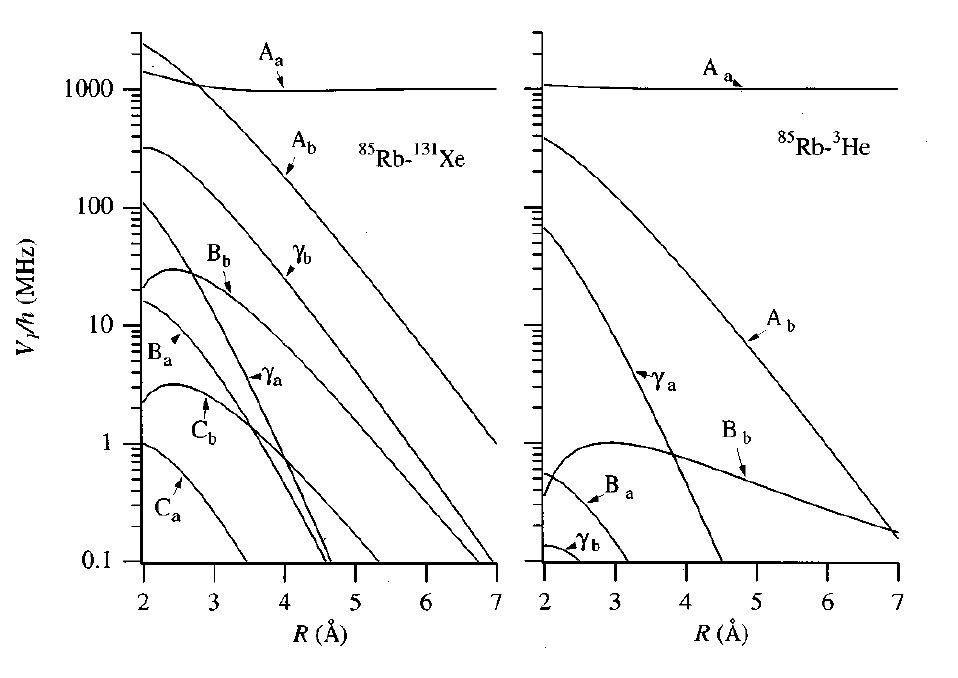
\includegraphics{V1.png}}
	\caption{{\bf Strengths of various spin-dependent interactions (from Ref.\@ \cite{WalkerHapper})}}
	\label{SpinExchange}
\end{figure}

\emph{et al.}
$\Delta F=\pm1$
$\vec{S}$

\addcontentsline{toc}{chapter}{Bibliography}
\bibliography{ref}

\end{document}